The results in section \ref{res:amazon} show that there is a linear correlation between performance and number of nodes for each scale above 15. 


\begin{figure}[!h]
	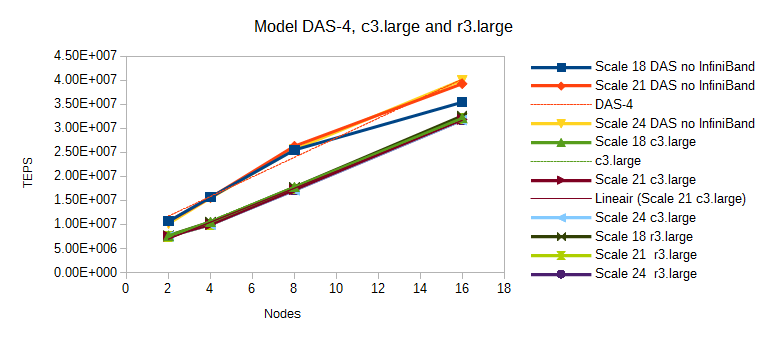
\includegraphics[width=\textwidth]{images/model_figure_1.png}
	\caption{The linear behavior for the DAS-4,c3.large and r3.large.}
	\label{fig:model_first}
\end{figure}

We general model will be:
\begin{equation}
\label{eq:model}
 TEPS(scale) = 
 \begin{cases} 
	 a * \# nodes + b \leq T & \text{if scale} > 15  \\ \text{slow decrease} > T & \text{if scale} > 15
 \end{cases}
\end{equation}
Where $T$ is the tipping point and is defined as: $T = f(scale, architecture)$. Equation \ref{eq:model} calculates the performance for given scale for a specific number of nodes.

\begin{table}[!h]
	\begin{center}

	\begin{tabular}{|l|l|l|}
		\hline
		Experiment & a (MTEPS) & b  (MTEPS)\\ \hline
		DAS-4 scale 21 & 2.03 & 7.70 \\ \hline
		DAS-4 scale 24 & 2.11 & 7.00 \\ \hline
		Amazon EC2 c3.large scale 21 & 1.76 & 3.45 \\ \hline
		Amazon EC2 c3.large scale 24 & 1.76 & 3.41 \\ \hline 
		Amazon EC2 r3.large scale 21 & 1.78 & 3.36 \\ \hline 
		Amazon EC2 r3.large scale 24 & 1.75 & 3.42 \\ \hline 
	\end{tabular}
	\end{center}
	\caption{The values for a and b from equation \ref{eq:model} for different scale and architectures.}
	\label{tab:model}
\end{table}
To calculate the a and b for a different architectures and scale, a regression line has been made for the  experiments seen in figure \ref{fig:model_first}. Table \ref{tab:model} shows the results of creating these regression line. The table show there is not much difference between the a and b on the same architecture. This means a more general formula can be created for each of the architectures. 

First the equation for the DAS-4:
\begin{equation}
\label{eq:das}
TEPS(scale) = 2.03 * x + 7.70
\end{equation}

Second the equation for Amazon EC2:
\begin{equation}
\label{eq:amazon}
TEPS(scale) = 1.76 * x + 3.45
\end{equation}
Where x is the number of nodes used for the application. Both equations return a value in $10^6$ TEPS (MTEPS).

As can be seen from these two equations the slope and the starting value depend on the architecture on which the Graph 500 benchmark runs. To calibrate the experiments at least 3 experiments need to be done with the hardware of choice. When a and b have been found the model is complete and a prediction can be made for different experiments.

The model made can only predict the performance of the as a function of the number of nodes for large scales. The point where maximum parallelism can be achieved and the point of the diminishing return cannot be calculated with equation \ref{eq:das} or \ref{eq:amazon}.